% ----------------------------------------------------------
% Capítulo 3 -- Análise do Sistema
% ----------------------------------------------------------
\chapter{Análise do Sistema}\label{cap:analise}

Este capítulo transforma a compreensão do contexto e das necessidades em uma visão estruturada do sistema a ser desenvolvido. Seu objetivo é definir o que o \textit{SyncCarreira} deve fazer, quem interage com ele, quais conceitos compõem seu domínio e quais requisitos e restrições devem ser considerados, sem incorporar decisões de implementação. Os requisitos aqui apresentados derivam do Documento de Requisitos do Sistema, negociado e assinado pela equipe e pela parceira do projeto (APÊNDICE A).

\section{Visão Geral do Sistema}\label{sec:visao-geral}

O \textit{SyncCarreira} é uma plataforma \textit{web}, estruturada no modelo \textit{Software as a Service} (SaaS), voltada à orientação vocacional de jovens vinculados a instituições parceiras, isto é, escolas e organizações não governamentais. O sistema organiza a jornada do jovem em cinco trilhas sequenciais e obrigatórias — autoconhecimento, influências, informação, projeto de futuro e síntese final —, compostas por questões de um banco fixo validado pelo profissional de orientação, e encerra cada trilha com o registro de uma síntese reflexiva. Ao término da jornada, apresenta ao aluno um leque de áreas e carreiras sugeridas, sempre como ponto de partida para reflexão.

Aos profissionais de orientação (psicólogos(as) e mentores(as) educacionais) o sistema oferece um painel de acompanhamento do progresso dos alunos, a sinalização dos casos que demandam atenção prioritária e recursos de agendamento de sessões, envio de \textit{feedback}, curadoria de fontes externas e emissão de relatórios. A plataforma não substitui a atuação desse profissional: seu papel é estruturar o acompanhamento e sinalizar prioridades, mantendo o conteúdo psicológico sob validação humana.

O sistema delimita-se a três perfis de acesso — Administrador, Profissional de Orientação e Aluno — e comunica-se com dois sistemas externos: um serviço de agenda (Google Calendar), responsável pelo envio dos convites das sessões de orientação, e um serviço de envio de mensagens eletrônicas, responsável pelas notificações. Os dados de cada instituição parceira permanecem isolados dos dados das demais.

\section{Atores Envolvidos}\label{sec:atores}

Um ator, em Engenharia de Requisitos, representa qualquer entidade externa — pessoa, sistema ou dispositivo — que interage diretamente com o sistema para realizar ou receber um serviço \cite{pressman2021}. Os atores primários iniciam a interação para alcançar um objetivo; os atores secundários prestam um serviço ao sistema durante a execução de um caso de uso.

O \autoref{quadro-atores} identifica os atores do \textit{SyncCarreira} e sintetiza seus papéis.

\begin{quadro}[H]
\ABNTEXfontereduzida
\caption{Atores do SyncCarreira.}
\label{quadro-atores}
\renewcommand{\arraystretch}{1.25}
\begin{tabularx}{\textwidth}{|>{\raggedright\arraybackslash}p{3.6cm}|>{\raggedright\arraybackslash}p{2.3cm}|>{\raggedright\arraybackslash}X|}
\hline
\textbf{Ator} & \textbf{Tipo} & \textbf{Descrição do papel} \\
\hline
Administrador & Primário & Configura o ambiente da plataforma: cadastra e gerencia as instituições parceiras e suas turmas, cria e mantém as contas dos profissionais de orientação e dos alunos e vincula cada aluno à sua turma. \\
\hline
Profissional de Orientação (psicólogo(a) ou mentor(a) educacional) & Primário & Acompanha o progresso dos alunos da instituição à qual está vinculado, identifica os alunos que sinalizaram dúvida, realiza a curadoria de fontes externas, agenda sessões de orientação, envia \textit{feedbacks} e emite relatórios. \\
\hline
Aluno (mentorado) & Primário & Protagonista da jornada: personaliza seu perfil de interesses, percorre as trilhas, registra suas sínteses e consulta seu leque de possibilidades, o panorama e o histórico de suas jornadas, seus agendamentos e os \textit{feedbacks} recebidos. \\
\hline
Google Calendar & Secundário (sistema externo) & Recebe os eventos das sessões de orientação, gera o \textit{link} de videoconferência e envia aos alunos convidados os convites, as atualizações e os cancelamentos. \\
\hline
Serviço de e-mail & Secundário (sistema externo) & Entrega as mensagens de primeiro acesso, os avisos de \textit{feedback} ao aluno e os alertas de sinalização de dúvida ao profissional de orientação. \\
\hline
\end{tabularx}
\legend{Fonte: Autoria própria (2026).}
\end{quadro}

Os comportamentos automáticos do sistema, como a sinalização de alunos em dúvida (RF-04) e a priorização desses alunos para atendimento (RN-04), não constituem um ator, pois são executados pelo próprio sistema em resposta às ações dos atores primários.

\section{Casos de Uso}\label{sec:casos-de-uso}

Um caso de uso descreve uma sequência de ações que um sistema executa para produzir um resultado observável e de valor para um ator específico \cite{pressman2021}. O \textit{SyncCarreira} possui dezesseis casos de uso. A autenticação (UC16) é pré-condição de todos os demais, uma vez que nenhuma funcionalidade é acessível sem que o usuário esteja identificado. A \autoref{fig_casos_uso} apresenta o diagrama de casos de uso.

\begin{figure}[H]
    \centering
    \caption{Diagrama de casos de uso do SyncCarreira.}
    \label{fig_casos_uso}
    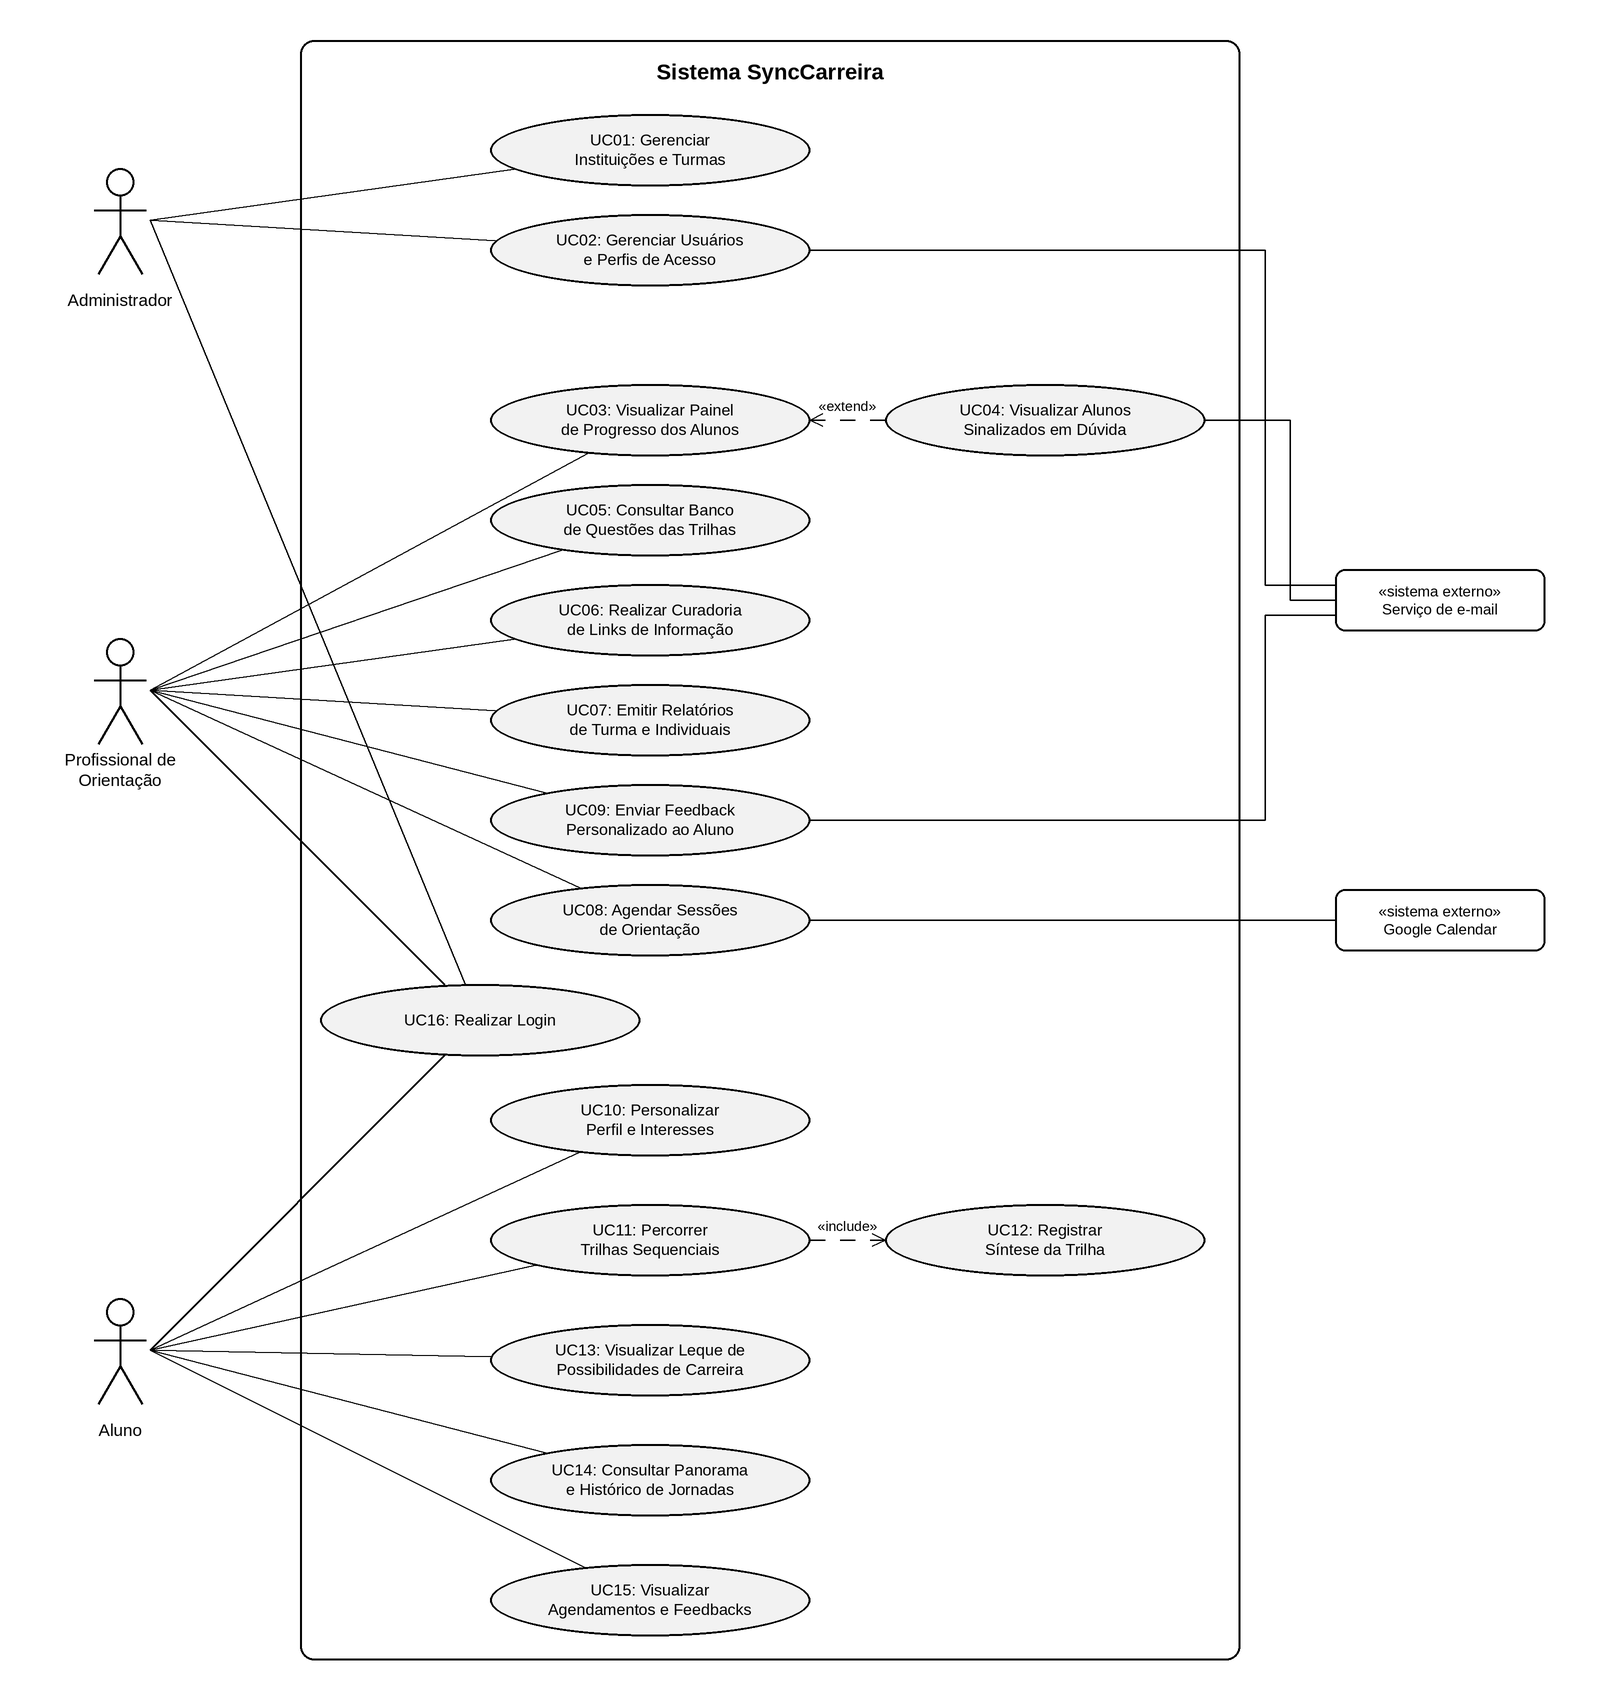
\includegraphics[width=0.95\textwidth]{img/fig-cap3-casos-de-uso.png}
    \legend{Fonte: Autoria própria (2026).}
\end{figure}

A seguir, cada caso de uso é detalhado em ator, requisitos relacionados, pré-condições, pós-condições, fluxo principal, fluxos alternativos (FA) e fluxos de exceção (FE).

\subsection*{UC01 -- Gerenciar Instituições e Turmas}\label{uc:uc01}

\textit{Ator principal:} Administrador.

\textit{Requisitos relacionados:} RF-01, RNF-08.

\textit{Descrição:} permite ao Administrador cadastrar, editar, ativar e desativar as instituições parceiras (escolas ou ONGs) e criar as turmas vinculadas a cada uma delas.

\textit{Pré-condições:} Administrador autenticado (UC16).

\textit{Pós-condições:} instituição registrada e apta a receber turmas, profissionais de orientação e alunos; turmas vinculadas a uma instituição ativa.

\textit{Fluxo principal:} (1) Administrador acessa o módulo de Gestão e seleciona a aba ``Instituições''; (2) sistema exibe a lista de instituições cadastradas, com CNPJ, tipo e situação (ativa ou inativa); (3) Administrador aciona o cadastro de nova instituição; (4) sistema exibe o formulário com razão social, nome fantasia, CNPJ e tipo de instituição (pública, particular ou ONG); (5) Administrador preenche os campos e confirma; (6) sistema valida os dados, registra a instituição como ativa e atualiza a lista.

\textit{Fluxos alternativos:}

\begin{itemize}[label={},leftmargin=\parindent,itemsep=0pt,topsep=0pt]
  \item FA01 – Editar instituição: Administrador seleciona uma instituição, altera seus dados e confirma; o sistema valida e atualiza o registro.
  \item FA02 – Ativar ou desativar instituição: Administrador altera a situação da instituição; uma instituição inativa deixa de estar disponível para o cadastro de turmas e o vínculo de profissionais de orientação.
  \item FA03 – Cadastrar turma: na aba ``Turmas'', Administrador informa o nome da turma, o ano letivo e a instituição; o sistema registra a turma vinculada à instituição.
\end{itemize}

\textit{Fluxos de exceção:}

\begin{itemize}[label={},leftmargin=\parindent,itemsep=0pt,topsep=0pt]
  \item FE01 – CNPJ inválido: o sistema informa a inconsistência e mantém o formulário aberto.
  \item FE02 – CNPJ já cadastrado: o sistema informa a duplicidade e impede o registro.
  \item FE03 – Campos obrigatórios não preenchidos: o sistema destaca os campos e impede o registro.
  \item FE04 – Turma vinculada a instituição inativa: o sistema impede o cadastro da turma.
\end{itemize}

\subsection*{UC02 -- Gerenciar Usuários e Perfis de Acesso}\label{uc:uc02}

\textit{Ator principal:} Administrador.

\textit{Atores secundários:} Serviço de e-mail.

\textit{Requisitos relacionados:} RF-02, RNF-01, RNF-02.

\textit{Descrição:} permite ao Administrador cadastrar, editar e desativar as contas de profissionais de orientação e de alunos, definindo o perfil de acesso de cada uma, e vincular os alunos às respectivas turmas.

\textit{Pré-condições:} Administrador autenticado (UC16); ao menos uma instituição ativa cadastrada.

\textit{Pós-condições:} conta criada com perfil de acesso definido e vinculada à instituição (profissional de orientação) ou à turma (aluno); mensagem de primeiro acesso enviada ao e-mail cadastrado.

\textit{Fluxo principal:} (1) Administrador acessa a aba ``Usuários'' e seleciona o perfil desejado (Aluno ou Profissional de Orientação); (2) sistema exibe as contas cadastradas nesse perfil; (3) Administrador aciona o cadastro de nova conta; (4) sistema exibe o formulário correspondente ao perfil: para o profissional de orientação, nome, e-mail, número de registro no Conselho Regional de Psicologia (CRP, opcional para mentores(as) sem registro), instituição e data de validade do contrato; para o aluno, nome, e-mail, ano escolar e tipo de escola; (5) Administrador preenche os campos e confirma; (6) sistema valida os dados, cria a conta com o perfil correspondente e envia ao e-mail informado uma mensagem de primeiro acesso com \textit{link} para definição de senha; (7) a nova conta passa a constar na listagem.

\textit{Fluxos alternativos:}

\begin{itemize}[label={},leftmargin=\parindent,itemsep=0pt,topsep=0pt]
  \item FA01 – Editar conta: Administrador seleciona a conta, altera os dados e confirma.
  \item FA02 – Vincular aluno a turma: Administrador seleciona o aluno, aciona ``Associar turma'' e escolhe uma das turmas cadastradas; o sistema registra o vínculo e, por consequência, a instituição do aluno.
  \item FA03 – Desativar conta: o sistema solicita confirmação e, por se tratar de exclusão definitiva em conformidade com a LGPD, remove a conta e os dados a ela associados.
\end{itemize}

\textit{Fluxos de exceção:}

\begin{itemize}[label={},leftmargin=\parindent,itemsep=0pt,topsep=0pt]
  \item FE01 – E-mail já cadastrado: o sistema informa a duplicidade e impede o registro.
  \item FE02 – Profissional de orientação já cadastrado com o mesmo nome e CRP: o sistema informa a duplicidade.
  \item FE03 – Nenhuma instituição ativa ou turma cadastrada: o sistema orienta o cadastro prévio (UC01).
\end{itemize}

\subsection*{UC03 -- Visualizar Painel de Progresso dos Alunos}\label{uc:uc03}

\textit{Ator principal:} Profissional de Orientação.

\textit{Requisitos relacionados:} RF-03, RN-03, RNF-01, RNF-08.

\textit{Descrição:} tela inicial do profissional de orientação; apresenta, em painel único, o progresso de cada aluno da instituição em cada trilha, sem exibir o conteúdo das respostas e das sínteses.

\textit{Pré-condições:} Profissional de orientação autenticado (UC16) e vinculado a uma instituição.

\textit{Pós-condições:} operação somente de leitura; nenhum dado é alterado.

\textit{Fluxo principal:} (1) após a autenticação, o sistema exibe o painel de progresso; (2) sistema apresenta os indicadores consolidados: total de alunos e quantidade de alunos com jornada não iniciada, em andamento, concluída e sinalizada em dúvida; (3) sistema apresenta a conclusão por etapa, isto é, a quantidade de alunos que concluiu cada trilha; (4) sistema lista os alunos com turma, etapa atual, percentual de progresso e situação da jornada; (5) profissional de orientação filtra a lista por nome, turma ou situação; (6) profissional de orientação expande a linha de um aluno; (7) sistema exibe o progresso do aluno por trilha: questões respondidas, percentual concluído e registro da síntese.

\textit{Fluxos alternativos:}

\begin{itemize}[label={},leftmargin=\parindent,itemsep=0pt,topsep=0pt]
  \item FA01 – Alunos sinalizados em dúvida: havendo alunos com sinalização ativa, executa-se o UC04.
\end{itemize}

\textit{Fluxos de exceção:}

\begin{itemize}[label={},leftmargin=\parindent,itemsep=0pt,topsep=0pt]
  \item FE01 – Nenhum aluno vinculado à instituição: o sistema informa que ainda não há alunos para exibir.
  \item FE02 – Profissional de orientação sem instituição vinculada: o sistema informa a pendência e não exibe o painel.
  \item FE03 – Nenhum aluno corresponde aos filtros: o sistema informa e mantém os filtros disponíveis para ajuste.
\end{itemize}

\textit{Relação UML:} ponto de extensão para o UC04 («extend»).

\subsection*{UC04 -- Visualizar Alunos Sinalizados em Dúvida}\label{uc:uc04}

\textit{Ator principal:} Profissional de Orientação.

\textit{Atores secundários:} Serviço de e-mail.

\textit{Requisitos relacionados:} RF-04, RF-05, RN-03, RN-04.

\textit{Descrição:} extensão do UC03. Quando um aluno conclui a jornada e sinaliza que permanece em dúvida quanto à escolha profissional, o sistema notifica automaticamente os profissionais de orientação da instituição e destaca o aluno no painel, priorizando-o para atendimento.

\textit{Pré-condições:} UC03 em execução; ao menos um aluno da instituição com sinalização de dúvida ativa.

\textit{Pós-condições:} profissional de orientação identificou os alunos prioritários e pode agendar uma sessão (UC08) ou enviar um \textit{feedback} (UC09).

\textit{Fluxo principal:} (1) quando o aluno sinaliza dúvida (UC13), o sistema registra a data da sinalização e envia mensagem eletrônica aos profissionais de orientação com contrato vigente na instituição do aluno; (2) no painel, o sistema exibe a seção ``Alunos que sinalizaram dúvida''; (3) profissional de orientação seleciona um aluno da seção; (4) sistema exibe o progresso detalhado do aluno; (5) profissional de orientação decide a ação: agendar uma sessão (UC08), restringindo a seleção aos alunos em dúvida, ou enviar um \textit{feedback} (UC09).

\textit{Fluxos alternativos:}

\begin{itemize}[label={},leftmargin=\parindent,itemsep=0pt,topsep=0pt]
  \item FA01 – Nenhuma sinalização ativa: o painel é exibido sem a seção de alunos em dúvida.
\end{itemize}

\textit{Fluxos de exceção:}

\begin{itemize}[label={},leftmargin=\parindent,itemsep=0pt,topsep=0pt]
  \item FE01 – Aluno sem turma vinculada ou instituição sem profissional com contrato vigente: a sinalização é registrada, mas nenhuma notificação é enviada.
\end{itemize}

\textit{Relação UML:} «extend» UC03.

\subsection*{UC05 -- Consultar Banco de Questões das Trilhas}\label{uc:uc05}

\textit{Ator principal:} Profissional de Orientação.

\textit{Requisitos relacionados:} RN-06, RN-09.

\textit{Descrição:} permite consultar, em modo somente de leitura, as questões e as opções de resposta do banco fixo de cada trilha, previamente aprovado e validado pelo profissional de orientação.

\textit{Pré-condições:} Profissional de orientação autenticado (UC16); banco de questões carregado no sistema.

\textit{Pós-condições:} operação somente de leitura.

\textit{Fluxo principal:} (1) profissional de orientação acessa a consulta do banco de questões; (2) sistema exibe as trilhas na ordem sequencial; (3) profissional de orientação seleciona uma trilha; (4) sistema exibe as questões da trilha, com o tipo de cada uma (múltipla escolha, múltipla seleção ou escala Likert) e as respectivas opções de resposta.

\textit{Fluxos de exceção:}

\begin{itemize}[label={},leftmargin=\parindent,itemsep=0pt,topsep=0pt]
  \item FE01 – Tentativa de alteração do conteúdo: o sistema não oferece edição ao profissional de orientação; alterações no banco de questões restringem-se ao Administrador, mediante validação do profissional de orientação.
\end{itemize}

\subsection*{UC06 -- Realizar Curadoria de Links da Trilha de Informação}\label{uc:uc06}

\textit{Ator principal:} Profissional de Orientação.

\textit{Atores secundários:} Aluno (consulta).

\textit{Requisitos relacionados:} RF-06, RN-05.

\textit{Descrição:} permite cadastrar e remover \textit{links} de fontes externas confiáveis — como Enem, ProUni, políticas de cotas e portais de cursos — exibidos ao aluno na trilha de Informação.

\textit{Pré-condições:} Profissional de orientação autenticado (UC16).

\textit{Pós-condições:} \textit{link} registrado e disponível na trilha de Informação.

\textit{Fluxo principal:} (1) profissional de orientação acessa a área ``Curadoria de links''; (2) sistema exibe as fontes cadastradas, com tópico, categoria e endereço; (3) profissional de orientação informa o tópico ou nome da fonte, o endereço (URL) e a categoria de exibição: ``ENEM, ProUni, cotas e ingresso'' ou uma das áreas do conhecimento (Humanas, Exatas, Biológicas ou Artes); (4) profissional de orientação confirma o cadastro; (5) sistema valida o endereço, registra o \textit{link} e atualiza a lista.

\textit{Fluxos alternativos:}

\begin{itemize}[label={},leftmargin=\parindent,itemsep=0pt,topsep=0pt]
  \item FA01 – Remover \textit{link}: profissional de orientação remove uma fonte, que deixa de ser exibida na trilha de Informação.
  \item FA02 – Exibição ao aluno: na trilha de Informação, o aluno visualiza, como materiais complementares de consulta opcional, os \textit{links} de acesso ao ensino superior e os \textit{links} das áreas do conhecimento em que obteve maior pontuação.
\end{itemize}

\textit{Fluxos de exceção:}

\begin{itemize}[label={},leftmargin=\parindent,itemsep=0pt,topsep=0pt]
  \item FE01 – Endereço inválido: o endereço não se inicia por http:// ou https://; o sistema informa e impede o registro.
  \item FE02 – Campos obrigatórios não preenchidos: o sistema destaca os campos e impede o registro.
\end{itemize}

\subsection*{UC07 -- Emitir Relatórios de Turma e Individuais}\label{uc:uc07}

\textit{Ator principal:} Profissional de Orientação.

\textit{Requisitos relacionados:} RF-07, RN-03.

\textit{Descrição:} permite gerar e baixar o relatório consolidado de uma turma e o relatório individual de um aluno, com dados cadastrais, pontuação por área, progresso nas trilhas e sínteses registradas.

\textit{Pré-condições:} Profissional de orientação autenticado (UC16); turma ou aluno pertencente à sua instituição.

\textit{Pós-condições:} relatório gerado em formato de planilha e disponível para \textit{download}.

\textit{Fluxo principal:} (1) profissional de orientação aciona a emissão de relatórios a partir do painel de progresso; (2) sistema oferece as opções de relatório de turma ou relatório individual; (3) profissional de orientação seleciona o tipo e a turma ou o aluno; (4) sistema consolida os dados e gera a planilha; (5) profissional de orientação baixa o arquivo.

\textit{Fluxos alternativos:}

\begin{itemize}[label={},leftmargin=\parindent,itemsep=0pt,topsep=0pt]
  \item FA01 – Relatório de turma: além dos dados individuais de cada aluno, apresenta o total de alunos e a distribuição por situação da jornada (não iniciada, em andamento, concluída e em dúvida).
\end{itemize}

\textit{Fluxos de exceção:}

\begin{itemize}[label={},leftmargin=\parindent,itemsep=0pt,topsep=0pt]
  \item FE01 – Turma ou aluno de outra instituição: o sistema nega o acesso.
\end{itemize}

\subsection*{UC08 -- Agendar Sessões de Orientação}\label{uc:uc08}

\textit{Ator principal:} Profissional de Orientação.

\textit{Atores secundários:} Aluno; Google Calendar.

\textit{Requisitos relacionados:} RF-05, RF-08, RN-04, RNF-08.

\textit{Descrição:} permite criar, editar e cancelar sessões de orientação individuais ou em grupo com alunos da instituição, com envio automático de convite ao aluno por meio do Google Calendar.

\textit{Pré-condições:} Profissional de orientação autenticado (UC16) e vinculado a uma instituição; ao menos um aluno vinculado a uma turma da instituição.

\textit{Pós-condições:} sessão registrada com situação ``agendada''; quando a conta do Google Agenda está conectada, evento criado na agenda do profissional de orientação, com \textit{link} de videoconferência, e convite enviado aos alunos.

\textit{Fluxo principal:} (1) profissional de orientação acessa a área ``Agendamentos''; (2) sistema exibe as sessões futuras e o histórico de sessões; (3) profissional de orientação conecta sua conta do Google Agenda, caso ainda não esteja conectada; (4) profissional de orientação aciona ``Nova sessão''; (5) sistema exibe o formulário com tipo de sessão (individual ou em grupo), alunos, título (opcional), data, horário, duração e pauta ou observações para o aluno; (6) profissional de orientação seleciona os alunos — podendo restringir a lista aos alunos sinalizados em dúvida — e confirma; (7) sistema valida os dados, cria o evento no Google Calendar com \textit{link} do Google Meet, tendo os alunos como convidados, e registra a sessão; (8) Google Calendar envia o convite por e-mail aos alunos.

\textit{Fluxos alternativos:}

\begin{itemize}[label={},leftmargin=\parindent,itemsep=0pt,topsep=0pt]
  \item FA01 – Editar sessão agendada: profissional de orientação altera os dados da sessão; o sistema atualiza o registro e o evento, e o Google Calendar envia a atualização aos convidados.
  \item FA02 – Cancelar sessão: profissional de orientação informa o motivo do cancelamento; o sistema registra a situação ``cancelada'', o motivo passa a ser visível ao aluno e o Google Calendar envia o cancelamento aos convidados.
  \item FA03 – Conta do Google Agenda não conectada: a sessão é registrada sem \textit{link} de videoconferência e sem convite automático.
\end{itemize}

\textit{Fluxos de exceção:}

\begin{itemize}[label={},leftmargin=\parindent,itemsep=0pt,topsep=0pt]
  \item FE01 – Sessão individual com número de alunos diferente de um: o sistema impede o registro.
  \item FE02 – Sessão em grupo com menos de dois alunos: o sistema impede o registro.
  \item FE03 – Aluno de outra instituição ou sem turma vinculada: o sistema nega o acesso.
  \item FE04 – Edição ou cancelamento de sessão já cancelada ou realizada: o sistema impede a operação.
\end{itemize}

\subsection*{UC09 -- Enviar Feedback Personalizado ao Aluno}\label{uc:uc09}

\textit{Ator principal:} Profissional de Orientação.

\textit{Atores secundários:} Aluno; Serviço de e-mail.

\textit{Requisitos relacionados:} RF-09.

\textit{Descrição:} permite redigir e enviar um \textit{feedback} textual individual ao aluno, ao final de uma jornada concluída ou após uma sessão de orientação da qual ele participou.

\textit{Pré-condições:} Profissional de orientação autenticado (UC16); aluno da sua instituição que concluiu a jornada ou que participou de sessão realizada.

\textit{Pós-condições:} \textit{feedback} registrado, disponível na área do aluno (UC15), e aluno notificado por e-mail.

\textit{Fluxo principal:} (1) profissional de orientação seleciona uma sessão realizada ou um aluno com jornada concluída; (2) aciona o envio de \textit{feedback}; (3) sistema exibe o campo de texto do \textit{feedback}; (4) profissional de orientação redige o texto, com até 5.000 caracteres, e confirma o envio; (5) sistema registra o \textit{feedback}, associando-o à sessão ou à jornada correspondente, e envia mensagem eletrônica ao aluno informando o recebimento.

\textit{Fluxos alternativos:}

\begin{itemize}[label={},leftmargin=\parindent,itemsep=0pt,topsep=0pt]
  \item FA01 – Feedback de sessão em grupo: o profissional de orientação envia um \textit{feedback} individual a cada aluno participante.
  \item FA02 – Consultar e excluir \textit{feedbacks} enviados: o profissional de orientação visualiza os \textit{feedbacks} já enviados, com a indicação de leitura pelo aluno, e pode excluí-los.
\end{itemize}

\textit{Fluxos de exceção:}

\begin{itemize}[label={},leftmargin=\parindent,itemsep=0pt,topsep=0pt]
  \item FE01 – Texto em branco: o sistema impede o envio.
  \item FE02 – Feedback já enviado ao aluno para a mesma jornada ou sessão: o sistema informa a duplicidade.
  \item FE03 – Sessão cancelada ou aluno que não participou da sessão: o sistema impede o envio.
\end{itemize}

\subsection*{UC10 -- Personalizar Perfil e Interesses}\label{uc:uc10}

\textit{Ator principal:} Aluno.

\textit{Requisitos relacionados:} RF-14.

\textit{Descrição:} permite ao aluno atribuir um grau de interesse, de 0 (``não me interessa'') a 5 (``tenho muito interesse''), a cada uma das quatro grandes áreas do conhecimento — Humanas, Exatas, Biológicas e Artes —, contextualizando a jornada. Os graus informados compõem a pontuação considerada no leque de possibilidades (UC13).

\textit{Pré-condições:} Aluno autenticado (UC16).

\textit{Pós-condições:} interesses registrados; no primeiro preenchimento, acesso às trilhas liberado.

\textit{Fluxo principal:} (1) no primeiro acesso, o sistema verifica que o perfil não foi preenchido e direciona o aluno a ``Meu perfil'' antes de liberar as trilhas; (2) sistema exibe as quatro áreas do conhecimento, cada uma com escala de 0 a 5; (3) aluno atribui uma nota a cada área; (4) aluno confirma; (5) sistema registra os interesses e recalcula a pontuação da jornada em andamento; (6) sistema libera o acesso às trilhas.

\textit{Fluxos alternativos:}

\begin{itemize}[label={},leftmargin=\parindent,itemsep=0pt,topsep=0pt]
  \item FA01 – Atualizar interesses durante a jornada: o aluno altera as notas a qualquer momento; o sistema recalcula a pontuação da jornada em andamento, sem alterar o resultado de jornadas já concluídas.
\end{itemize}

\textit{Fluxos de exceção:}

\begin{itemize}[label={},leftmargin=\parindent,itemsep=0pt,topsep=0pt]
  \item FE01 – Área sem nota atribuída: o sistema impede o registro.
  \item FE02 – Tentativa de abrir uma trilha sem o perfil preenchido: o sistema direciona o aluno a ``Meu perfil''.
\end{itemize}

\subsection*{UC11 -- Percorrer Trilhas Sequenciais}\label{uc:uc11}

\textit{Ator principal:} Aluno.

\textit{Requisitos relacionados:} RF-10, RN-01, RN-09.

\textit{Descrição:} permite ao aluno percorrer as cinco trilhas da jornada na ordem obrigatória; cada trilha libera a seguinte somente após concluída, isto é, com todas as questões respondidas e a síntese registrada.

\textit{Pré-condições:} Aluno autenticado (UC16); perfil preenchido (UC10); para as trilhas seguintes à primeira, trilha anterior concluída.

\textit{Pós-condições:} respostas registradas; trilha concluída após o registro da síntese (UC12).

\textit{Fluxo principal:} (1) sistema exibe as trilhas com sua situação (bloqueada, disponível, em andamento ou concluída) e o progresso de cada uma; (2) aluno seleciona a trilha disponível; (3) sistema verifica a liberação da trilha e exibe suas questões; (4) aluno responde às questões, apresentadas nos formatos de múltipla escolha, múltipla seleção ou escala Likert; cada resposta é registrada no momento em que é informada; (5) sistema atualiza o progresso da trilha; (6) respondidas todas as questões, o sistema exibe o campo de síntese (UC12).

\textit{Fluxos alternativos:}

\begin{itemize}[label={},leftmargin=\parindent,itemsep=0pt,topsep=0pt]
  \item FA01 – Interromper e retomar: o aluno deixa a trilha e, no acesso seguinte, retoma do ponto em que parou, com as respostas preservadas.
  \item FA02 – Alterar resposta: enquanto a trilha estiver em andamento, uma nova resposta à mesma questão substitui a anterior.
  \item FA03 – Trilha de Informação: além das questões, o sistema apresenta os \textit{links} curados pelo profissional de orientação (UC06), como materiais complementares de consulta opcional.
\end{itemize}

\textit{Fluxos de exceção:}

\begin{itemize}[label={},leftmargin=\parindent,itemsep=0pt,topsep=0pt]
  \item FE01 – Tentativa de acessar trilha bloqueada: o sistema informa que é necessário concluir a trilha anterior, incluindo sua síntese.
\end{itemize}

\textit{Relação UML:} «include» UC12.

\subsection*{UC12 -- Registrar Síntese da Trilha}\label{uc:uc12}

\textit{Ator principal:} Aluno.

\textit{Atores secundários:} Profissional de Orientação (consulta posterior, por meio de relatório).

\textit{Requisitos relacionados:} RF-11, RN-02.

\textit{Descrição:} ao concluir as questões de cada trilha, o aluno registra obrigatoriamente uma síntese reflexiva em texto livre, sem restrição de conteúdo, condição para a conclusão da trilha e a liberação da seguinte.

\textit{Pré-condições:} todas as questões da trilha respondidas (UC11).

\textit{Pós-condições:} síntese registrada; trilha concluída e trilha seguinte liberada.

\textit{Fluxo principal:} (1) sistema exibe o campo de texto livre da síntese; (2) aluno redige a síntese; (3) aluno aciona ``Salvar e concluir trilha''; (4) sistema verifica que o texto não está em branco e que respeita o limite de 5.000 caracteres; (5) sistema registra a síntese com a data do registro; (6) sistema marca a trilha como concluída e libera a trilha seguinte.

\textit{Fluxos alternativos:}

\begin{itemize}[label={},leftmargin=\parindent,itemsep=0pt,topsep=0pt]
  \item FA01 – Síntese final da jornada: na última trilha, o registro da síntese conclui a jornada, que passa a constar no histórico do aluno, e o sistema disponibiliza o leque de possibilidades (UC13).
\end{itemize}

\textit{Fluxos de exceção:}

\begin{itemize}[label={},leftmargin=\parindent,itemsep=0pt,topsep=0pt]
  \item FE01 – Síntese em branco: o sistema impede o registro.
  \item FE02 – Questões pendentes: o sistema impede o registro e informa que todas as questões devem ser respondidas.
  \item FE03 – Síntese já registrada: o sistema impede novo registro ou alteração da síntese daquela trilha.
\end{itemize}

\textit{Relação UML:} incluído pelo UC11 («include»).

\subsection*{UC13 -- Visualizar Leque de Possibilidades de Carreira}\label{uc:uc13}

\textit{Ator principal:} Aluno.

\textit{Atores secundários:} Serviço de e-mail.

\textit{Requisitos relacionados:} RF-12, RF-04, RN-07.

\textit{Descrição:} após a conclusão da jornada, apresenta ao aluno um conjunto de áreas do conhecimento e de carreiras compatíveis com suas respostas e interesses, sempre como ponto de partida para reflexão, e nunca como diagnóstico fechado.

\textit{Pré-condições:} Aluno autenticado (UC16); jornada concluída (UC12).

\textit{Pós-condições:} aluno visualizou seu leque de possibilidades; opcionalmente, sinalizou dúvida.

\textit{Fluxo principal:} (1) concluída a jornada, o aluno aciona ``Ver meu leque de carreiras''; (2) sistema calcula, para cada área do conhecimento, o percentual da pontuação obtida em relação à máxima possível, considerando os interesses declarados (UC10) e os pesos das opções de resposta escolhidas; (3) sistema exibe as quatro áreas em ordem decrescente de percentual, destacando as de maior percentual, inclusive em caso de empate; (4) para as áreas em destaque, o sistema apresenta subáreas do conhecimento, com breve descrição e exemplos de carreiras; (5) sistema exibe o aviso de que o resultado constitui ponto de partida para reflexão, e não diagnóstico de carreira.

\textit{Fluxos alternativos:}

\begin{itemize}[label={},leftmargin=\parindent,itemsep=0pt,topsep=0pt]
  \item FA01 – Sinalizar dúvida: o aluno indica que permanece em dúvida quanto à escolha profissional; o sistema registra a sinalização e notifica os profissionais de orientação (UC04).
  \item FA02 – Consultar o leque de uma jornada anterior: a partir do histórico (UC14), o aluno visualiza o resultado registrado no momento da conclusão daquela jornada.
\end{itemize}

\textit{Fluxos de exceção:}

\begin{itemize}[label={},leftmargin=\parindent,itemsep=0pt,topsep=0pt]
  \item FE01 – Jornada não concluída: o sistema informa que o resultado ainda não está disponível.
  \item FE02 – Dúvida já sinalizada: o sistema informa que a sinalização já foi registrada.
\end{itemize}

\subsection*{UC14 -- Consultar Panorama e Histórico de Jornadas}\label{uc:uc14}

\textit{Ator principal:} Aluno.

\textit{Requisitos relacionados:} RF-13, RF-15, RN-08.

\textit{Descrição:} permite ao aluno consultar, a qualquer momento, as respostas e sínteses da jornada em andamento e as jornadas concluídas em ciclos anteriores, acompanhando sua evolução ao longo do tempo.

\textit{Pré-condições:} Aluno autenticado (UC16); perfil preenchido (UC10).

\textit{Pós-condições:} operação de leitura; opcionalmente, nova jornada iniciada.

\textit{Fluxo principal:} (1) aluno acessa ``Minha jornada''; (2) sistema exibe, para a jornada em andamento, cada etapa percorrida com as respostas informadas e a síntese registrada; (3) sistema indica as etapas ainda não percorridas; (4) sistema exibe as jornadas concluídas anteriormente, com número, data de conclusão, turma, instituição e áreas em destaque; (5) aluno seleciona uma jornada concluída para consultar suas respostas, sínteses e resultado.

\textit{Fluxos alternativos:}

\begin{itemize}[label={},leftmargin=\parindent,itemsep=0pt,topsep=0pt]
  \item FA01 – Baixar jornada concluída: o aluno baixa, em formato PDF, o registro de uma jornada concluída.
  \item FA02 – Iniciar nova jornada: concluída a jornada atual, o aluno inicia um novo ciclo; o sistema preserva a jornada concluída no histórico e reinicia as trilhas.
\end{itemize}

\textit{Fluxos de exceção:}

\begin{itemize}[label={},leftmargin=\parindent,itemsep=0pt,topsep=0pt]
  \item FE01 – Nenhuma jornada concluída: o sistema informa que as jornadas concluídas serão exibidas nessa área.
  \item FE02 – Tentativa de iniciar nova jornada com a atual em andamento: o sistema impede a operação.
\end{itemize}

\subsection*{UC15 -- Visualizar Agendamentos e Feedbacks}\label{uc:uc15}

\textit{Ator principal:} Aluno.

\textit{Atores secundários:} Profissional de Orientação.

\textit{Requisitos relacionados:} RF-16.

\textit{Descrição:} permite ao aluno consultar, em área própria, as sessões de orientação para as quais foi convocado (UC08) e os \textit{feedbacks} recebidos (UC09).

\textit{Pré-condições:} Aluno autenticado (UC16).

\textit{Pós-condições:} operação de leitura; \textit{feedbacks} abertos registrados como lidos.

\textit{Fluxo principal:} (1) aluno acessa ``Agendamentos''; (2) sistema exibe as próximas sessões, com data, horário, duração, tipo e pauta; (3) quando disponível, o aluno acessa a videoconferência ou adiciona a sessão à sua agenda; (4) sistema exibe o histórico de sessões realizadas e canceladas; (5) sistema exibe os \textit{feedbacks} recebidos do profissional de orientação; (6) ao abrir um \textit{feedback}, o sistema o registra como lido.

\textit{Fluxos alternativos:}

\begin{itemize}[label={},leftmargin=\parindent,itemsep=0pt,topsep=0pt]
  \item FA01 – Nenhuma sessão futura: o sistema informa a ausência de agendamentos e mantém os \textit{feedbacks} disponíveis para consulta.
\end{itemize}

\textit{Fluxos de exceção:}

\begin{itemize}[label={},leftmargin=\parindent,itemsep=0pt,topsep=0pt]
  \item FE01 – Sessão cancelada pelo profissional de orientação: o sistema exibe a situação ``cancelada'' e o motivo informado.
\end{itemize}

\subsection*{UC16 -- Realizar Login}\label{uc:uc16}

\textit{Ator principal:} Administrador, Profissional de Orientação e Aluno.

\textit{Atores secundários:} Serviço de e-mail (primeiro acesso).

\textit{Requisitos relacionados:} RNF-01.

\textit{Descrição:} garante a autenticação de qualquer usuário, verificando suas credenciais e estabelecendo a sessão conforme o perfil de acesso; constitui pré-condição de todos os demais casos de uso.

\textit{Pré-condições:} usuário cadastrado (UC02).

\textit{Pós-condições:} sessão autenticada estabelecida, com tempo de validade limitado e com as permissões do perfil; usuário direcionado à tela inicial correspondente.

\textit{Fluxo principal:} (1) usuário acessa a plataforma; (2) sistema exibe a tela de autenticação; (3) usuário informa e-mail e senha; (4) sistema valida as credenciais; (5) sistema identifica o perfil de acesso; (6) sistema estabelece a sessão e direciona o usuário à tela inicial do perfil: painel de progresso, para o profissional de orientação; trilhas, para o aluno; gestão, para o Administrador.

\textit{Fluxos alternativos:}

\begin{itemize}[label={},leftmargin=\parindent,itemsep=0pt,topsep=0pt]
  \item FA01 – Primeiro acesso: por meio do \textit{link} recebido por e-mail no cadastro (UC02), o usuário define sua senha, com no mínimo oito caracteres e confirmação, dentro do prazo de validade do \textit{link}; em seguida, realiza a autenticação.
  \item FA02 – Esquecimento de senha: o sistema orienta o usuário a procurar o Administrador ou o profissional de orientação de sua instituição.
\end{itemize}

\textit{Fluxos de exceção:}

\begin{itemize}[label={},leftmargin=\parindent,itemsep=0pt,topsep=0pt]
  \item FE01 – Credenciais inválidas: o sistema exibe mensagem genérica, sem indicar qual dado está incorreto.
  \item FE02 – \textit{Link} de primeiro acesso inválido ou expirado: o sistema impede a definição da senha.
  \item FE03 – Senha com menos de oito caracteres ou confirmação divergente: o sistema impede a definição da senha.
\end{itemize}

\section{Modelo Conceitual}\label{sec:modelo-conceitual}

O modelo conceitual representa os principais conceitos do domínio do problema, seus atributos e relacionamentos, sem incorporar decisões de implementação, como tipos de dados, chaves ou mecanismos de persistência. Na modelagem orientada a objetos, essa representação é construída por meio de classes de análise, que descrevem as entidades relevantes do domínio, e das associações entre elas, com as respectivas multiplicidades \cite{pressman2021}. A \autoref{fig_classes_conceitual} apresenta o diagrama de classes conceitual do \textit{SyncCarreira}.

\begin{figure}[H]
    \centering
    \caption{Diagrama de classes conceitual do SyncCarreira.}
    \label{fig_classes_conceitual}
    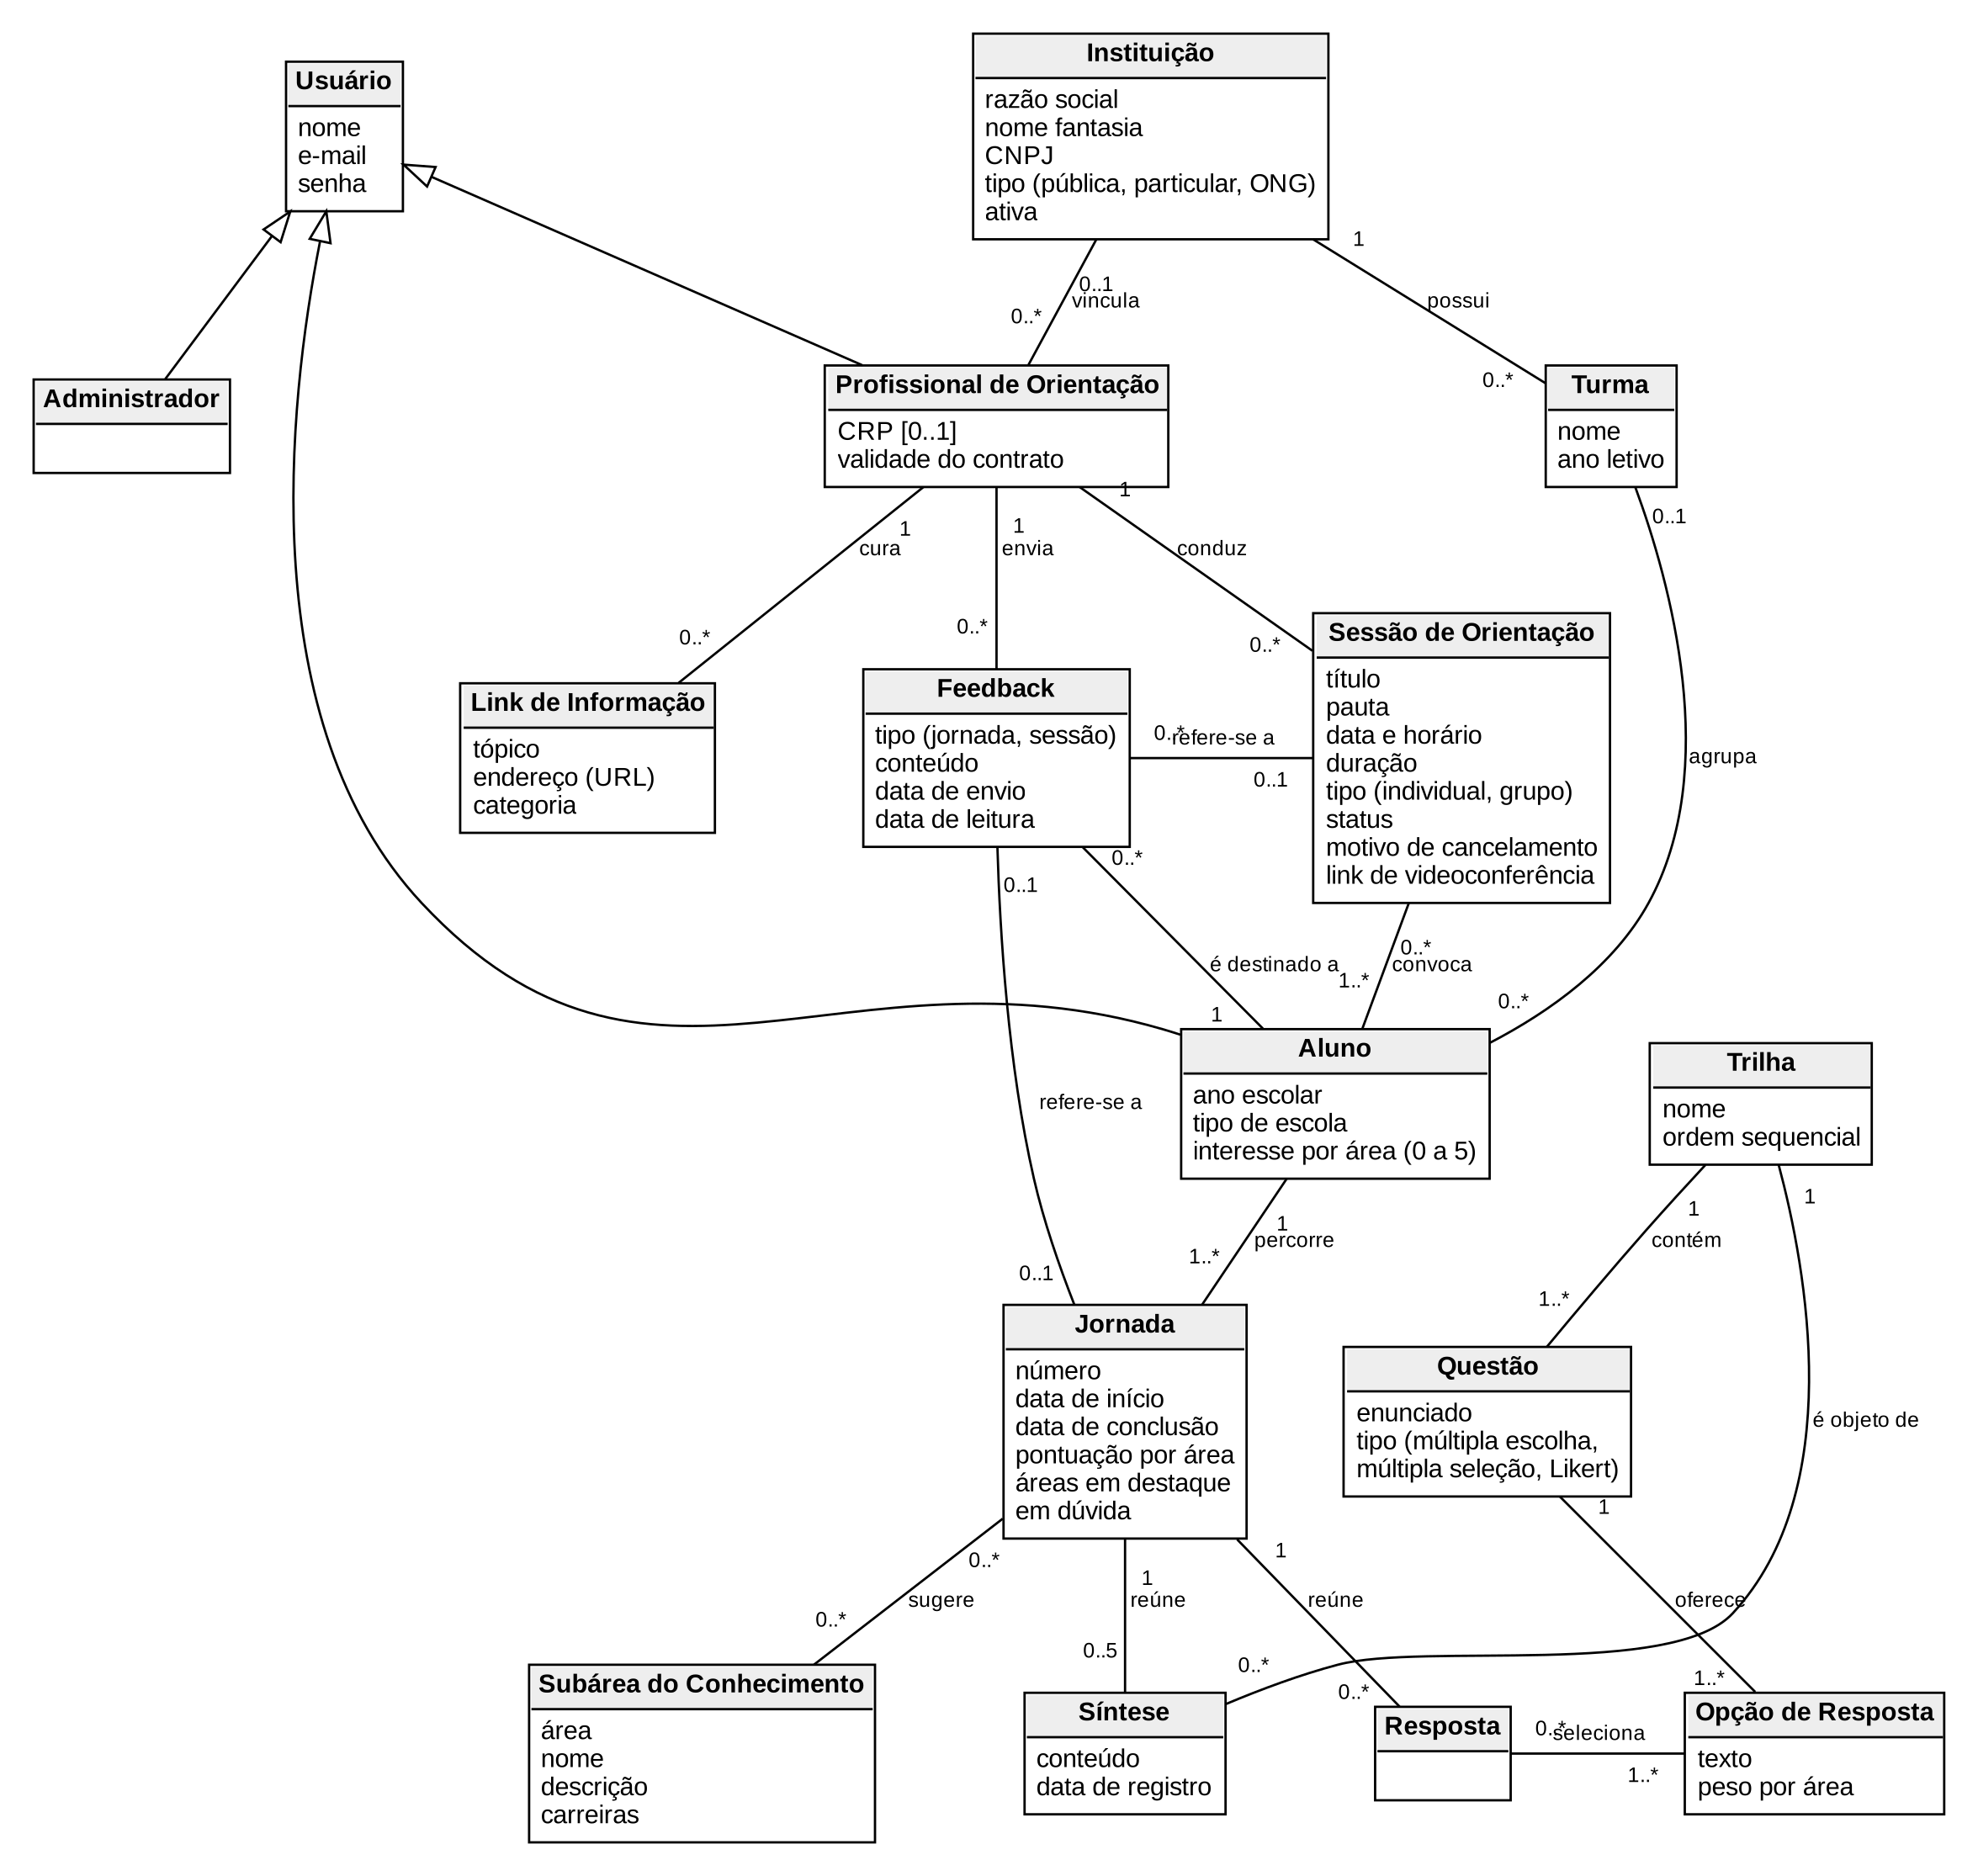
\includegraphics[width=\textwidth]{img/fig-cap3-classes-conceitual.png}
    \legend{Fonte: Autoria própria (2026).}
\end{figure}

A partir desse diagrama, destacam-se os seguintes conceitos:

\begin{itemize}
  \item \textbf{Usuário}: conceito geral que se especializa em Administrador, Profissional de Orientação e Aluno;
  \item \textbf{Instituição}: escola ou ONG parceira, unidade de isolamento dos dados;
  \item \textbf{Turma}: agrupamento de alunos vinculado a uma Instituição, identificado por nome e ano letivo;
  \item \textbf{Profissional de Orientação}: psicólogo(a) ou mentor(a) educacional vinculado a uma Instituição, com registro no CRP opcional;
  \item \textbf{Aluno}: participante da jornada, caracterizado pelo ano escolar, pelo tipo de escola e pelo grau de interesse declarado em cada área do conhecimento;
  \item \textbf{Jornada}: ciclo completo de orientação percorrido pelo Aluno, que reúne suas Respostas e Sínteses e registra a pontuação por área, as áreas em destaque e a eventual sinalização de dúvida;
  \item \textbf{Trilha}: etapa sequencial da jornada, composta por Questões;
  \item \textbf{Questão} e \textbf{Opção de Resposta}: itens do banco fixo de questões; cada opção atribui pesos às áreas do conhecimento;
  \item \textbf{Resposta}: seleção, pelo Aluno, de uma ou mais Opções de Resposta;
  \item \textbf{Síntese}: texto reflexivo registrado pelo Aluno ao final de cada Trilha;
  \item \textbf{Subárea do Conhecimento}: desdobramento de uma área do conhecimento, com descrição e exemplos de carreiras, sugerido ao final da Jornada;
  \item \textbf{Link de Informação}: fonte externa curada pelo Profissional de Orientação e exibida na trilha de Informação;
  \item \textbf{Sessão de Orientação}: encontro individual ou em grupo, conduzido por um Profissional de Orientação e com um ou mais Alunos convocados;
  \item \textbf{Feedback}: mensagem textual enviada pelo Profissional de Orientação a um Aluno, referente a uma Jornada concluída ou a uma Sessão de Orientação.
\end{itemize}

\section{Requisitos Funcionais}\label{sec:rf}

Um requisito funcional é uma declaração sobre um serviço que o sistema deve fornecer, descrevendo como ele deve reagir a entradas específicas e como deve se comportar em determinadas situações \cite{pressman2021}. \citeonline{sommerville2011} acrescenta que os requisitos funcionais podem, em alguns casos, explicitar também o que o sistema não deve fazer — caso da vedação a diagnósticos fechados de carreira no \textit{SyncCarreira}.

O \autoref{quadro-rf} apresenta os dezesseis requisitos funcionais do sistema, organizados por ator responsável.

\begin{quadro}[H]
\ABNTEXfontereduzida
\caption{Requisitos funcionais do SyncCarreira.}
\label{quadro-rf}
\renewcommand{\arraystretch}{1.25}
\begin{tabularx}{\textwidth}{|>{\centering\arraybackslash}p{1.2cm}|>{\raggedright\arraybackslash}p{3.6cm}|>{\raggedright\arraybackslash}X|}
\hline
\textbf{ID} & \textbf{Requisito} & \textbf{Descrição} \\
\hline
\multicolumn{3}{|l|}{\cellcolor{gray!12}\textbf{Administrador}} \\
\hline
RF-01 & Gestão de instituições & Cadastrar e gerenciar escolas/ONGs, vinculando usuários e turmas a cada instituição. \\
\hline
RF-02 & Gestão de usuários e perfis & Criar, editar e desativar contas de profissionais de orientação e alunos, definindo o perfil de acesso de cada um. \\
\hline
\multicolumn{3}{|l|}{\cellcolor{gray!12}\textbf{Profissional de Orientação}} \\
\hline
RF-03 & Painel de status por aluno & Visualizar em um painel único o progresso de cada aluno em cada trilha. \\
\hline
RF-05 & Priorização de alunos em dúvida & Filtrar alunos sinalizados com dúvida e agendá-los para atendimento individual ou em grupo. \\
\hline
RF-06 & Curadoria de links externos & Cadastrar links de fontes confiáveis (Enem, ProUni, cotas, cursos) para exibição na trilha de Informação. \\
\hline
RF-07 & Relatórios de turma e individuais & Baixar relatório geral da turma e relatórios individuais com sínteses e status de cada aluno. \\
\hline
RF-08 & Agendamento de sessões & Criar, editar e cancelar sessões individuais ou em grupo, com aviso ao aluno pelo Google Calendar. \\
\hline
RF-09 & Feedback personalizado & Enviar feedback textual ao aluno ao final da jornada ou após uma sessão de orientação. \\
\hline
\multicolumn{3}{|l|}{\cellcolor{gray!12}\textbf{Sistema (automático)}} \\
\hline
RF-04 & Alerta de necessidade de orientação & Sinalizar automaticamente, no painel do profissional de orientação, alunos que concluíram as trilhas com dúvida ou indecisão. \\
\hline
\multicolumn{3}{|l|}{\cellcolor{gray!12}\textbf{Aluno}} \\
\hline
RF-10 & Jornada de 5 trilhas em ordem & Percorrer as trilhas na sequência obrigatória: autoconhecimento $\rightarrow$ influências $\rightarrow$ informação $\rightarrow$ projeto de futuro $\rightarrow$ síntese. Cada trilha só libera a próxima após concluída. \\
\hline
RF-11 & Síntese ao final de cada trilha & Registrar um texto livre com reflexões e conclusões ao concluir cada trilha, sem restrição de conteúdo. \\
\hline
RF-12 & Leque de carreiras sugeridas & Ver, ao final da jornada, um conjunto de áreas e carreiras sugeridas, sempre como ponto de partida, nunca como diagnóstico fechado. \\
\hline
RF-13 & Panorama da jornada & Consultar a qualquer momento o histórico de respostas e sínteses das trilhas já concluídas. \\
\hline
RF-14 & Personalização de perfil & Configurar informações de perfil e interesses para contextualizar a jornada. \\
\hline
RF-15 & Histórico de jornadas anteriores & Consultar jornadas de ciclos anteriores, acompanhando sua evolução ao longo do tempo. \\
\hline
RF-16 & Agendamentos e feedbacks & Ver, em uma área própria, os agendamentos de sessão e os feedbacks enviados pelo profissional de orientação. \\
\hline
\end{tabularx}
\legend{Fonte: Autoria própria (2026).}
\end{quadro}

\section{Requisitos Não Funcionais}\label{sec:rnf}

Os requisitos não funcionais são restrições sobre os serviços ou as funções oferecidos pelo sistema, relacionadas a atributos de qualidade como desempenho, segurança, disponibilidade e usabilidade, e frequentemente se aplicam ao sistema como um todo, e não a uma funcionalidade isolada \cite{pressman2021}. \citeonline{sommerville2011} organiza esses requisitos em três categorias: requisitos de produto, que especificam o comportamento do \textit{software}, como velocidade de execução e confiabilidade; requisitos organizacionais, decorrentes de políticas e procedimentos da organização cliente; e requisitos externos, originados de fatores alheios ao sistema e a seu processo de desenvolvimento, como exigências legais e regulatórias. No \textit{SyncCarreira}, os requisitos RNF-01, RNF-03, RNF-04, RNF-06, RNF-07 e RNF-08 são requisitos de produto; o RNF-05 aproxima-se de um requisito organizacional, vinculado ao horário de funcionamento das instituições parceiras; e o RNF-02, decorrente da Lei Geral de Proteção de Dados Pessoais (LGPD), é um requisito externo.

O \autoref{quadro-rnf} apresenta os oito requisitos não funcionais do sistema.

\begin{quadro}[H]
\ABNTEXfontereduzida
\caption{Requisitos não funcionais do SyncCarreira.}
\label{quadro-rnf}
\renewcommand{\arraystretch}{1.25}
\begin{tabularx}{\textwidth}{|>{\centering\arraybackslash}p{1.4cm}|>{\raggedright\arraybackslash}p{3.6cm}|>{\raggedright\arraybackslash}X|}
\hline
\textbf{ID} & \textbf{Categoria} & \textbf{Descrição} \\
\hline
RNF-01 & Segurança (autenticação e autorização) & Cada usuário só acessa as ferramentas permitidas ao seu perfil; um aluno não vê informações de outros alunos, e um profissional de orientação só acessa suas próprias turmas. \\
\hline
RNF-02 & Privacidade e proteção de dados (LGPD) & Dados sensíveis (respostas, sentimentos e perfis) são armazenados com criptografia; o sistema garante a exclusão total dos dados mediante solicitação do aluno ou da instituição. \\
\hline
RNF-03 & Desempenho (tempo de resposta) & Ações cotidianas, como carregar uma trilha ou salvar uma resposta, levam no máximo 2 segundos em condições normais de uso. \\
\hline
RNF-04 & Usabilidade (interface acessível e responsiva) & Interface responsiva, construída com abordagem \textit{mobile-first}, com navegação intuitiva o suficiente para dispensar manual de instruções. \\
\hline
RNF-05 & Disponibilidade & Plataforma disponível pelo menos 99\% do tempo durante o horário letivo (7h às 22h em dias úteis); manutenções programadas fora desse horário. \\
\hline
RNF-06 & Manutenibilidade (arquitetura em camadas) & Arquitetura organizada em camadas, de modo a permitir a adição futura de funcionalidades sem necessidade de refatoração completa. \\
\hline
RNF-07 & Documentação de API & Interface de programação do sistema documentada automaticamente, viabilizando futuras integrações com sistemas escolares de terceiros. \\
\hline
RNF-08 & Isolamento de dados por instituição & Dados de alunos, turmas, trilhas e resultados de uma instituição nunca se misturam ou ficam visíveis para outra instituição cadastrada. \\
\hline
\end{tabularx}
\legend{Fonte: Autoria própria (2026).}
\end{quadro}

\section{Restrições do Sistema}\label{sec:restricoes}

Além dos requisitos funcionais e não funcionais, todo projeto de \textit{software} está sujeito a restrições: condições impostas externamente ao processo de desenvolvimento que limitam as escolhas de projeto, como prazo, orçamento, tecnologia obrigatória ou decisões deliberadas sobre o que permanece fora do escopo de uma versão do produto \cite{pressman2021}. A norma ISO/IEC/IEEE 29148:2018 trata essas restrições como requisitos de projeto e implementação (\textit{design and implementation requirements}), categoria que abrange limitações de instalação, distribuição, portabilidade, reusabilidade, custo e prazo \cite{iso29148-2018}. Diferentemente de um requisito funcional ou não funcional, uma restrição não descreve o que o sistema deve fazer ou como deve se comportar, mas o que ele explicitamente não fará na versão em desenvolvimento, o que contribui para alinhar as expectativas entre a equipe e a instituição parceira.

O Documento de Requisitos do Sistema delimita quatro exclusões de escopo que operam como restrições ao desenvolvimento do \textit{SyncCarreira}:

\begin{enumerate}[label=\alph*)]
  \item \textbf{Validação clínica e metodologia psicológica}: a responsabilidade da equipe técnica restringe-se à entrega da infraestrutura tecnológica. O projeto não contempla a criação de novos instrumentos psicométricos proprietários, tampouco a homologação ou validação clínica junto ao Conselho Federal de Psicologia (CFP); a validação do sistema utiliza lógicas de orientação de domínio público ou dados simulados, e o fornecimento do conteúdo final é de responsabilidade da instituição parceira.
  \item \textbf{Publicação de aplicativos nativos}: a plataforma é entregue como aplicação \textit{web} responsiva, projetada para funcionar em navegadores de \textit{smartphones} e \textit{tablets}; o desenvolvimento e a publicação de aplicativos nativos nas lojas App Store e Play Store não estão previstos nesta versão.
  \item \textbf{Módulo financeiro e \textit{gateway} de pagamentos}: embora a arquitetura seja projetada para um modelo de negócio SaaS, esta versão não contempla fluxos de faturamento, integrações com \textit{gateways} de cartão de crédito, emissão de boletos ou de notas fiscais.
  \item \textbf{Integração com plataformas de terceiros}: o \textit{SyncCarreira} opera de forma independente, sem integrações automatizadas ou sincronização de dados com sistemas de gestão acadêmica ou ambientes virtuais de aprendizagem já utilizados pelas instituições de ensino; o provisionamento de contas e turmas ocorre por cadastro direto na plataforma.
\end{enumerate}
